\documentclass[12pt,a4paper]{article}
\usepackage[utf8]{inputenc}
\usepackage{amsmath}
\usepackage{amsfonts}
\usepackage{amssymb}
\usepackage{graphicx}
\usepackage[margin = 1in]{geometry}

%DRAWINGS
\usepackage{tikz}
\usepackage{circuitikz} % For electric circuits
%subfigure
\usepackage{caption}
\usepackage{subcaption}

%no indent
\setlength\parindent{0pt}

\usepackage{xparse}% http://ctan.org/pkg/xparse

% custom commands
\newcommand{\diver}[1]{\nabla \cdot} % derivative wrt t
\newcommand{\dt}[1]{\frac{d #1}{dt}} % derivative wrt t
\newcommand{\der}[2]{\frac{d #1}{d #2}} % derivative
\newcommand{\pd}[2]{\frac{\partial #1}{\partial #2}} % partial derivative
\newcommand{\integral}[3]{\int_{#1}^{#2} d #3 \ } % integral	

\newcommand{\tr}{\text{tr}}

\makeatletter
\def\overUnderArrow{\@ifnextchar[\overUnderArrow@i{\overUnderArrow@i[]}}
\def\overUnderArrow@i[#1]#2#3{% #1 under #2 over #3 main argument
  \ifx\relax#1\relax\array[b]{c}\overset{\text{#2}}{\uparrow}\\#3\endarray
  \else\ifx\relax#2\relax
    \array[t]{c}#3\\\underset{\text{#1}}{\downarrow}\endarray
  \else
    \array{c}\overset{\text{#2}}{\uparrow}\\#3\\\underset{\text{#1}}{\downarrow}\endarray
  \fi\fi}
\makeatother



\author{José Antonio}
\begin{document}
\section{Gauge Theory}
\textbf{Gauge Transformation}\\
Local transformation that leaves the Lagrangian/Hamiltonian unchaged.


Schrödinger equation is invariant under global transformations of the wave function
\begin{equation}
	\psi \rightarrow \psi'=e^{i\theta}\psi
\end{equation} 
Electrodynamics can be derived from a gauge transformation of the wave function
\begin{equation}
	\psi \rightarrow \psi'=e^{i\theta(t,x)}\psi
\end{equation} 
we write
\begin{equation}
	\theta(t,x) \equiv \frac{q}{\hbar c}\Lambda(t,x)
\end{equation}
Schrödinger eq. is invariant under a gauge transformation of the wave function by introducing the gauge fields $\vec{A}$ and $\varphi$ satisfying the transformations
\begin{eqnarray}
	\vec{A}' & = & \vec{A} + \nabla \Lambda \\
	\varphi' & = & \varphi - \frac{1}{c}\frac{\partial \Lambda}{\partial t}
\end{eqnarray}
We define the gauge invariant fields
\begin{eqnarray}
	\vec{B} & = & \nabla \times \vec{A} \\
	\vec{E} & = & - \nabla \varphi  - \frac{1}{c}\frac{\partial \vec{A}}{\partial t}
\end{eqnarray}
The \textit{magnetic field} $\vec{B}$ does no work. The power we need to move a particle subject to a Lorentz force, i.e. against the fields is
\begin{equation}
	P = -q\vec{E}\cdot \vec{v}
\end{equation}
We define the current of charge particles as
\begin{equation}
	I = \vec{j}\cdot \Delta \vec{S}
\end{equation}
\begin{eqnarray}
	 nq  = & \rho &  \text{charge density}\\\vec{j}  = & \rho \vec{v}  &  \text{current density}
\end{eqnarray}


\textbf{Lorenz Force}\\
In the presence of electric and magnetic fields, a particle with mass $m$ and charge $q$ expirience a force given by
\begin{equation}
	\vec{F} = q(\vec{E} + \frac{\vec{v}}{c}\times \vec{B})
\end{equation}

ALL CONSERVATION LAWS HAVE TO BE \emph{LOCAL} in order to respect the relativity of simultaneity.

\textbf{Conservation of charge}
\begin{equation}
	\dt{Q_V} + \int_{\partial V}{\vec{j}\cdot d\vec{a}} = 0
\end{equation}

\textbf{Generic conservation law}
\begin{equation}
\dt{C_V} + \int_{\partial V}{\overUnderArrow[density flux]{}{\vec{j}}\cdot d\vec{a}} = \overUnderArrow[sources within $V$]{}{F_V}
\end{equation}

\textbf{Conservation of energy}

\begin{equation}
\frac{d}{dt}\int_V d^3\vec{r} \ u + \int_{\partial V}d\vec{a} \cdot \vec{S} = -  \int_V d^3 \vec{r} \  \vec{j} \cdot \vec{E}
\end{equation}
where $u = \frac{E^2+B^2}{8\pi}$ is the e-m energy density  and $\vec{S}=\frac{c}{4\pi}\vec{E}\times \vec{B}$ is the Poynting vector.

\textbf{Maxwell equations}
\begin{eqnarray}
	\nabla \cdot \vec{B} & = & 0 \\
	\nabla \times \vec{E} & = & -\frac{1}{c}\frac{\partial \vec{B}}{\partial t} \\ 
	\nabla \cdot \vec{E} & = & 4 \pi \rho \\
	\nabla \times \vec{B} & = &\frac{4\pi}{c}\vec{j} +\frac{1}{c}\frac{\partial \vec{E}}{\partial t}
\end{eqnarray}
\begin{center}
\begin{tabular}{ | p{0.15\textwidth} | p{0.45\textwidth}| p{.4\textwidth} | } 
\hline 
Gauss's law & \begin{equation}
\integral{\partial V}{}{\vec{a}\cdot \vec{E}} = 4\pi\integral{V}{}{^3r} \rho
\end{equation} &  \begin{center}
The flux of $\vec{E}$ through a closed surface equals the enclosed charge.
\end{center} \\ 
\hline 
-- & \begin{equation}
\integral{\partial V}{}{\vec{a}\cdot \vec{B}} = 0
\end{equation} & \begin{center}
	Magnetic charges are absent.
\end{center}  \\ 
\hline 
Faraday's law & \begin{equation}
\oint_C d\vec{r} \cdot \vec{E} = -\int_S d\vec{a} \cdot \frac{1}{c}\pd{\vec{B}}{t}
\end{equation} & \begin{center}
A varying magnetic flux generates an electromotive force.
\end{center} \\ 
\hline 
Ampere's law & \begin{equation}
\oint_C d\vec{r} \cdot \vec{B} = \int_S d\vec{a}\cdot\left( \frac{4\pi}{c}\vec{j}+\frac{1}{c}\pd{\vec{E}}{t} \right) 
\end{equation}  & The circulation of $\vec{B}$
 along a closed curve $C$ bordering a surface $S$ equals the flux thorugh $S$ the sum of hte usual current plus Maxwell's displacement current $\frac{1}{c}\pd{\vec{E}}{t} $. \\ 
\hline 
\end{tabular} 

\end{center}
\textbf{Helmohltz Theorem}

\textbf{Equations for the potentials}
\begin{eqnarray}
	\nabla^2 \varphi + \frac{1}{c}\frac{\partial}{\partial t}\nabla\cdot \vec{A} & = & -4\pi\rho \\	
	\nabla^2\vec{A} - \nabla \left( \nabla\cdot \vec{A}+ \frac{1}{c}\frac{\partial \varphi}{\partial t}\right)-\frac{1}{c^2}\frac{\partial^2  \vec{A}}{\partial t^2} & = & -\frac{4\pi}{c}\vec{j}
\end{eqnarray}
\textbf{Gauge Fixing}
\begin{eqnarray}
	\text{\textbf{Lorenz}}& \nabla \cdot \vec{A} \equiv & - \frac{1}{c}\frac{\partial \varphi}{\partial t} \\
	\text{\textbf{Coulomb}}& \nabla \cdot \vec{A} \equiv & 0\\
	\text{\textbf{Hamilton}} & \varphi \equiv & 0 \\
	\text{\textbf{Landau}} & A_x \equiv & 0 \text{ (Quantum Hall Effect)}
\end{eqnarray}

Using the Lorenz gauge
\begin{eqnarray}
\nabla^2 \varphi - \frac{1}{c^2}\frac{\partial^2}{\partial t^2}\varphi & = & -4\pi\rho \\	
	\nabla^2\vec{A}-\frac{1}{c^2}\frac{\partial^2  \vec{A}}{\partial t^2} & = & -\frac{4\pi}{c}\vec{j}
\end{eqnarray} 

Using the Coulomb gauge
\begin{eqnarray}
\nabla^2 \varphi  & = & -4\pi\rho \\	
	\nabla^2\vec{A}-\frac{1}{c^2}\frac{\partial^2  \vec{A}}{\partial t^2} & = & -\frac{4\pi}{c}\vec{j}_{\rm  T}
\end{eqnarray} 

In Coulomb's gauge and applying the fourier transform in the spatial derivatives
\begin{equation}
	\underbrace{\frac{d^2 A_k^{\alpha}}{dt^2}= -k^2c^2 A_k^{\alpha}}_{\text{Harm. osc.} \\ \omega_k = kc}  +  \underbrace{4\pi c j_k^{\alpha}}_{\text{Ext. rest. force}}
\end{equation}

\textbf{Casimir Effect}\\
Consider in the vaccum two perfect mirrors in front of each other at a distance $L$. Inside the mirrors suppose there is a potential $\vec{A}$. Each mode have a wave lenght given by the boudary conditions and can only take discrete values
\begin{equation}
	\lambda = \frac{2L}{m}, \Rightarrow k =\frac{m \pi}{L}, \, m = 1,2,\dots
\end{equation}
Each of these modes have an energy
\begin{equation}
	\epsilon_m = \hbar \omega_m (n_{m,\alpha} + 1/2) = \frac{\hbar m\pi c}{L} (n_{m,\alpha} + 1/2)\ ,
\end{equation}
$n$ counts photons ---not a well defined quantity---, $m$ enumarates modes and $\alpha =1,2$ enumerates the degrees of freedom. The total energy is then
\begin{equation}
	U = \sum_{m\alpha} \frac{\hbar m\pi c}{L}(\langle n_{m,\alpha}\rangle + 1/2) \ .
\end{equation}
In the lowest energy state with temperature $T = 0$ we have no photons $n = 0$. Thus, the energy is
\begin{equation}
	U = 2\sum_ m  \frac{\hbar m\pi c}{2L} \ = -\frac{\hbar \pi c}{12 L} \ .
\end{equation}
And the force
\begin{equation}
	F = -\frac{d}{dL} U (L) = - \frac{\hbar \pi c}{12L^2}
\end{equation}
The apparance of an atractive force between the mirrors is called the \textit{Casimir effect}.

\textbf{Pahse differences}\\

\textbf{Aharonov-Bohm Effect}\\
Suppose a double slit experiment with electrons, between the double slti and the screen we put a solenoid with a current circulating in the azimuthal direction. Inside the solenoid there is a magnetic field $\vec{B} \neq 0$, but outside $\vec{B} = 0$.

Over trajewctory $\mathcal{L}_{1,2}$ we have $\vec{B}=\nabla \times \vec{A} = 0 \Rightarrow \vec{A} =  \nabla \Lambda_{1,2} \Rightarrow \Lambda_{1,2} = \int\limits_{I\rightarrow F \text{ over } \mathcal{L}_{1,2}}{}{d\vec{l}\cdot\vec{A}}$. Let $\Psi_{01,02}$ be the wave function of an electron when $\vec{B}$ is off over trajectory $\mathcal{L}_{1,2}$. When $\vec{B}$ is on the wave function $\Psi_{01,02}$ become $\Psi_{1,2}$
\begin{equation}
	\Psi_{01,02} \rightarrow \Psi_{1,2} \propto e^{ikL_{1,2}+ \frac{q}{\hbar c}\Lambda_{1,2}}
\end{equation}
a phase difference in the fringe pattern appears
\begin{equation}
	 \Delta \varphi = k\Delta L +\frac{q}{\hbar c}(\Lambda_1 - \Lambda_2)
\end{equation}
where
\begin{equation}
\Lambda_1 - \Lambda_2 = \oint d \vec{l} \cdot \vec{A} = \int d\vec{a} \ \nabla \times \vec{A} = \Phi_B
\end{equation}
The shift in the fringe pattern i a double slit experiment in a region where $\vec{B} = 0$ is called the \textit{Aharonov-Bohm effect}. 

\begin{figure}[h]
	\centering
	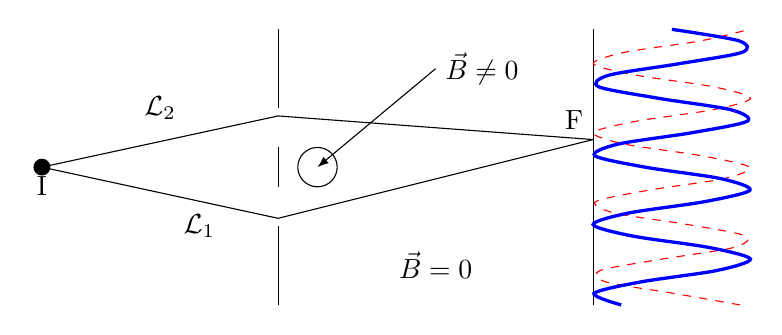
\begin{tikzpicture}
		% double slit
		\draw (0,0)--(0,0.5);
		\draw (0,1)--(0,2);
		\draw (0,-0.5)--(0,-1.5);
		
		% solenoid
		\draw (0.5,0.25) circle(0.25);
		
		%screen
		\draw (4,2) -- (4,-1.5);
		
		
		%source
		\draw[fill] (-3,0.25) node[below] {I} circle(0.1);
		
		%rays
		\draw (-3,0.25) -- (0,0.9)--(4,0.6) node [above left] {F};
		\draw (-3,0.25) -- (0,-0.4)--(4,0.6);

		%PATHS NAMES		
		\draw (-1,-0.5) node[] {$\mathcal{L}_1$};		
		\draw (-1.5,1) node[] {$\mathcal{L}_2$};
		
		%B values
		\draw (2,-1) node[] {$\vec{B} = 0$};
		\draw[latex-] (0.5,0.25)--(2,1.5) node[right] {$\vec{B} \neq 0$};
		
		%Intensity of fringes
		\draw[domain=-1.5:2, smooth, variable=\y, red,dashed]  plot ({sin(\y*400)+5}, {\y});
		\draw[domain=-1.5:2, smooth, variable=\y, blue,line width = 1.2]  plot ({sin(\y*400 + 100)+5}, {\y});
	\end{tikzpicture}
	\caption{Thick, $\vec{B}$ off. Dashed, $\vec{B}$ on.}
\end{figure}

\section{Electrostatics}
\textbf{Electric Field of a point charge}\\
\begin{equation}
	\vec{E}(\vec{r}\ ) = \frac{q}{r^3}\vec{r}
\end{equation}
\textbf{Dirac Delta function}\\
\begin{equation}
	\int_{-\infty}^{\infty} \frac{dk}{2\pi} \ e^{ik(x-x')} = \delta (x'-x)
\end{equation}

\textbf{Work to move a charge against $\vec{E}$}\\
\begin{equation}
	W = -q \int_{C'}d\vec{l} \cdot\vec{E}(\vec{r}\ ) 
\end{equation}
\textbf{Potential of a point charge due to $\vec{E}$}\\
\begin{equation}
	\varphi (\vec{r}\ ) = - \int_{\vec{O}}^{\vec{r}} d\vec{l} \cdot\vec{E}(\vec{r}\ ) 
\end{equation}
\textbf{Charged cylinder}\\

\textbf{Charged plane}\\
Consider a square plane of length $a$ with a charge $q$, then its superficial charge density is $\sigma = \frac{q}{a^2}$ 

\textbf{Charged plaque}\\ 

\textbf{Capacitance and capacitors}\\
The capacitance $C$ is the ability of a body to hold charge. And it is defined through
\begin{equation}
	Q= CV
\end{equation}
A capacitor is a device that stores energy in a electrical field.

\textbf{Poisson's Equation}\\

\textbf{Theorem} Let $\rho(\vec{r}) \in V$ and the potential in the boundary is given $F(\vec{r}\,)=\varphi(\vec{r} \,) \in \partial V$, then the potential in the volume $\varphi(\vec{r}\,), \  \vec{r} \in  V$ is unique. \\
\textit{Proof: }\\
Suppose $\varphi_1$ and $\varphi_2$ are two different solutions of Laplace equation and $\varphi_1 = \varphi_2 = F$ in the boundary. Let $\Psi = \varphi_2-\varphi_1$, then $\nabla^2 \Psi = 0$  and  $\Psi = 0$ in the boundary. Then
\begin{equation}
	\integral{V}{}{^3r} |\nabla \Psi|^2 = \integral{V}{}{^3r} \nabla\cdot (\Psi \nabla \Psi)- \integral{V}{}{^3r} \nabla^2 \Psi = \integral{\partial V}{}{ \vec{a}} \cdot \Psi\nabla \Psi = 0
\end{equation}
therefore $|\nabla \Psi|^2 = 0, \  \forall \vec{r} \in V  \Rightarrow \nabla \Psi = 0 \Rightarrow \Psi = \text{cte.}$  Thus $\Psi = 0$. QED.

\textbf{Theorem} Let $\rho(\vec{r}) \in V$ and the directional derivative ---along the perpendicular of the volume--- of the potential in the boundary is given $D(\vec{r}\,)=\partial_n\varphi(\vec{r} \,) \in \partial V$, then the potential in the volume $\varphi(\vec{r}\,), \  \vec{r} \in  V$ is unique up to a constant term. \\
\textit{Proof: }\\
Suppose $\varphi_1$ and $\varphi_2$ are two different solutions of Laplace equation and $\partial_n\varphi_1 = \partial_n\varphi_2 =D$ in the boundary. Let $\Psi = \varphi_2-\varphi_1$, then $\nabla^2 \Psi = 0$  and  $\partial_n\Psi = 0$ in the boundary. Then
\begin{equation}
	\integral{V}{}{^3r} |\nabla \Psi|^2 = \integral{\partial V}{}{ \vec{a}} \cdot \Psi\nabla \Psi =\integral{\partial V}{}{a} \cdot (\hat{n}\nabla \Psi)\Psi =\integral{\partial V}{}{a} (\partial_n \Psi)\Psi = 0 
\end{equation}
therefore $\nabla \Psi = 0 \Rightarrow \Psi = \text{cte.}$  Thus $\varphi_2 = \varphi_1 + \text{cte.}$ QED.

\textbf{Neumman and Dirchlet Boundary Conditions}\\

\textbf{Spontaneous Symmetry Breaking}\\


\textbf{Green's function}\\
Let $G(\vec{r},\vec{r}\,')$ be such that
\begin{equation}
	(\nabla')^2 G(\vec{r},\vec{r}\,') = -4\pi \delta (\vec{r}-\vec{r}\,')
\end{equation}

\begin{eqnarray}
	\varphi(\vec{r}) & = & \integral{V}{}{^3r'}\varphi(\vec{r}\,')\delta(\vec{r}-\vec{r}\,') = -\frac{1}{4\pi}\integral{V}{}{^3r'} \varphi(\vec{r}\,')(\nabla')^2 G(\vec{r},\vec{r}\,')\nonumber\\
	& = & -\frac{1}{4\pi}\integral{V}{}{^3r'} \nabla'\cdot \left( \varphi(r') \nabla' G(\vec{r},\vec{r}\,')\right) + \frac{1}{4\pi}\integral{V}{}{^3r'} (\nabla' \varphi(r'))\cdot \nabla' G(\vec{r},\vec{r}\,') \nonumber\\
	& = & -\frac{1}{4\pi} \int_{\partial V}d\vec{a} \cdot \varphi(\vec{r}\,')\nabla'G(\vec{r},\vec{r}\,') + \frac{1}{4\pi}\integral{V}{}{^3r'}\nabla'\cdot(\nabla'\varphi(\vec{r}\,'))G(\vec{r},\vec{r}\,')\nonumber\\
	& & -\frac{1}{4\pi}\integral{V}{}{^3r'}((\nabla')^2\varphi(\vec{r}\,')) G(\vec{r},\vec{r}\,')\\
	& = & -\frac{1}{4\pi} \integral{\partial V}{}{a}  \varphi(\vec{r}\,')\partial_{n'}G(\vec{r},\vec{r}\,') + \frac{1}{4\pi}\integral{\partial V}{}{a}G(\vec{r},\vec{r}\,')\partial_{n'}\varphi (\vec{r}\,') \\
	& & + \integral{V}{}{^3r'} G(\vec{r},\vec{r}\,') \rho(\vec{r}\,')
\end{eqnarray}

\textbf{Dirichlet Green's Function}\\
If we have Dirichlet's boundary conditions then 
\begin{equation}
	\varphi(\vec{r}) = \integral{V}{}{^3r'}G_D(\vec{r},\vec{r}\,') \rho(\vec{r}) -\frac{1}{4\pi} \integral{\partial V}{}{a}  \varphi(\vec{r}\,')\partial_{n'}G_D(\vec{r},\vec{r}\,')
\end{equation}
\textbf{Neumann Green's Function}\\
With Neumann boundary conditions, having $\partial_{n'} G_N(\vec{r},\vec{r}\,') = 0,\ \vec{r}\,'\in \partial V$ doesn't work since
\begin{equation}
	\integral{\partial V}{}{a'} \partial_{n'}G(\vec{r},\vec{r}\,') = -4\pi
\end{equation}
The next easiest ansatz for $G_N$ is a constant. Let $\partial_{n'} G_N = K = $ cte. Then
\begin{equation}
	\integral{\partial V}{}{a'} \partial_{n'}G(\vec{r},\vec{r}\,') = KA = -4\pi \Rightarrow K = -\frac{4\pi}{A}
\end{equation}
where $A$ is the area of the region. And finally
\begin{equation}
	\varphi(\vec{r}\,') = \integral{V}{}{^3r'} G_N(\vec{r},\vec{r}\,') + \langle \varphi \rangle_A + \frac{1}{4\pi}\integral{\partial V}{}{a'} G_N(\vec{r},\vec{r}\,') \partial_{n'} \varphi(\vec{r}\,')
\end{equation}
where $\langle \varphi \rangle_A = \frac{1}{A}\integral{\partial V}{}{a'} \varphi(\vec{r}\,')$ is the average of $\varphi$ over the surface.

\textbf{Green's function in Quantum Mechanics}\\

\textbf{Method of images}\\


\textbf{Green's function in spherical coordinates}\\
\begin{equation}
	G(\vec{r},\vec{r}\,') = \sum_{lm}\frac{4\pi}{2l+1} \frac{r_<^l}{r_>^{l+1}} Y_{lm}^*(\Omega)Y_{lm}(\Omega\,') = \frac{1}{|\vec{r}-\vec{r}\,'|}
\end{equation}

\textbf{Dipolar Electric moment}\\
\begin{equation}
	\vec{p} = \integral{}{}{^3r} \rho (\vec{r}\,)\vec{r}
\end{equation}

Potential
\begin{equation}
	\varphi(\vec{r}\,) = -\vec{p}\cdot \nabla\frac{1}{r} = \frac{\vec{p}\cdot \vec{r}}{r}
\end{equation}
Electric field
\begin{equation}
	\vec{E}(\vec{r}\,) =  \frac{3\vec{p}\cdot \vec{r} \ \vec{r}-\vec{p}r^2}{r^5}
\end{equation}
\textbf{Charge distribution of an electric dipole}\\
\begin{equation}
	\rho(\vec{r}\,) = -\vec{p} \cdot \nabla \delta (\vec{r}\,)
\end{equation}
\textbf{Polarization}\\
We define the polarization $\vec{P}$ as the density of electric dipole moments in a continous system with volume $V$
\begin{equation}
	\vec{P} \equiv \frac{\Delta \vec{p}}{\Delta V} 
\end{equation}
Let a tiny volume $\Delta V$ at $\vec{r}_0$ have a dipole moment $\Delta \vec{p}$ and a charge density $\Delta \rho^{\text{int}}$, then
\begin{equation}
	\Delta \rho^{\text{int}} = -\Delta \vec{p}  \cdot \nabla \delta (\vec{r} -\vec{r}_0) = - P(\vec{r}\,) \cdot \nabla \delta (\vec{r} -\vec{r}_0) 
\end{equation}
Integrating over the volume we get
\begin{equation}
 \rho^{\text{int}} = -\diver{} \vec{P}
\end{equation}
\textbf{Macroscopic Maxwell equations}\\

\textbf{Baoundary conditions}\\

\textbf{Energy of a system of charges}\\
	\begin{eqnarray}
		U & = & \frac{1}{2}\sum_{i\neq j} \frac{q_iq_j}{r_{ij}} \\
		& = & \sum_{i<j}\frac{q_iq_j}{r_{ij}}
	\end{eqnarray}

\textbf{Energy of a cointinous charge distribution}\\
\begin{equation}
	U = \frac{1}{2} \integral{}{}{^3r}\rho(\vec{r}\,) \varphi (\vec{r}\,)
\end{equation}
\textbf{Energy of a dipole}\\
\begin{equation}
	U = \vec{p} \cdot \nabla \varphi = -\vec{p} \cdot \vec{E}
\end{equation}

\textbf{Density matrix}\\
Pure state
\begin{equation}
	\vec{\rho} = |\Psi \rangle \langle \Psi|
\end{equation}
\begin{eqnarray}
	\langle  \hat{O} \rangle = \langle \Psi | \hat{O}|\Psi \rangle & = & \sum_{nm} \langle \Psi |n \rangle \langle n | \hat{O}|m \rangle\langle m  |\Psi  \rangle \\
	& = & \sum_{nm}  \langle n | \hat{O}|m \rangle\langle m  |\Psi  \rangle \langle \Psi |n \rangle \\
	& = &\sum_{nm} O_{nm}\rho_{mn} = \sum_{nmk} (O_{nm}\rho_{mk})\delta_{km}\\
	& = & \sum_{nk} (O\rho)_{nk}\delta_{kn} = \sum_{n} (\hat{O}\hat{\rho})_{nn} \\
	& = & \text{tr}(\hat{O}\hat{\rho})
\end{eqnarray}
\begin{equation}
	\hat{\rho} = \sum_{\Psi_{\alpha}}p_{\alpha} |\Psi_{\alpha} \rangle \langle \Psi_{\alpha}|
\end{equation}

\textbf{Schroedinger equation Interaction Scheme}\\
\begin{equation}
	i\hbar\partial_t \hat{O}_I = i\hbar \dt{\hat{O}} + [\hat{O},\hat{H}]
\end{equation}

\textbf{Evolution of $\hat{\rho}$ in interaction scheme} \\
Consider an interaction Hamiltonian term of the form $H_I = \zeta \hat{A}(t)\varphi(t)$. Then the Schoredinger equation reads
\begin{equation}
	i\hbar\partial_t \hat{\rho}(t) = \zeta [\hat{A}(t),\hat{\rho}]\varphi
\end{equation}
Integrating the equation
\begin{equation}
	\hat{\rho}(t) = \frac{1}{i\hbar} \integral{-\infty}{t}{t'} \zeta [\hat{A}(t'),\hat{\rho}(t)]\varphi(t') + \hat{\rho}_0
\end{equation}
where $\hat{\rho}_0$ is the matrix density in equilibrium, and we have assumed that $\varphi(t\rightarrow - \infty) = 0$.
Using perturbation theory we assume a solution of the form
\begin{equation}
	\hat{\rho}(t) =  \hat{\rho}_0 +\zeta\hat{\rho}^{(1)}(t) +\zeta^2\hat{\rho}^{(2)}(t) + \cdots
\end{equation}
So we get a solution
\begin{equation}
	\hat{\rho}^{(n+1)}(t) = \frac{1}{i\hbar}\integral{-\infty}{t}{t'}[\hat{A}(t'                                                                                                                           ),\hat{\rho}^{(n)}(t')]\varphi(t')
\end{equation}

\textbf{Response}\\
Consider a operator $\hat{B}$ subject to an inteaction $H_I$ defined as before. Then at  first approximation the expectation value of $\hat{B}$ is 
\begin{eqnarray}
	  \langle \hat{B}(t) \rangle^{(1)} & = & \text{tr}\left(\hat{\rho}^{(1)}(t                                                                                                                                                                                    )B(t)\right) \\
	  & = & \frac{1}{i\hbar}\integral{-\infty}{t}{t'}\text{tr}\left(\hat{B}(t)[\hat{A}(t'),\hat{\rho}_0]\right)\varphi(t')
\end{eqnarray}
Then we define the response as
\begin{equation}
	\chi_{BA}(t-t') = \frac{1}{i\hbar} \text{tr}\left(\hat{B}(t)[\hat{A}(t),\hat{\rho}_0]\right) \Theta(t-t')
\end{equation}
Use $\tr \left(O_1 [O_2,O_3] \right) = \tr \left([O_1,O_2]O_3 \right)$ to rewrite it as
\begin{equation}
\chi_{AB}(\tau) = \frac{1}{i\hbar}\langle [\hat{B}(\tau),\hat{A}(0)]\rangle_0 \Theta(\tau)
\end{equation}
where the subscript 0 means that it is computed at equilibrium.

\textbf{Polarizability}\\
Suppose an electron that is interacting with an electric dipole with energy $H_I = -\hat{d}_I(t) \cdot \hat{E}(t) = e\hat{r}(t)\cdot\hat{E}$. We identify $\hat{A}\rightarrow -\hat{d}= e\hat{r}(t)$. And we define $d(t) = \langle \hat{d}_I(t) \rangle$. We define the polarizability $\alpha$ trough
\begin{equation}
	d^i = \integral{}{}{t'} \alpha^{ij}(t-t')E^j(t')
\end{equation}
I we identufy $\hat{B} \rightarrow \hat{d}=-e\hat{r}$, then
 \begin{equation}
 	\alpha^{ij}(\tau) = -\frac{e^2}{i\hbar}\langle [\hat{r_I}^i(\tau),\hat{r_I}^j(0)]\rangle_0 \Theta(\tau)
 \end{equation}
Applying fourier transform 
\begin{equation}
	d_{\omega}^i = \alpha_{\omega}^{ij} E_{\omega}^j
\end{equation}
\begin{eqnarray}
	\alpha_{\omega}^{ij} & = & \integral{-\infty}{\infty}{\tau} \alpha^{ij}(\tau) e^{i(\omega+i\eta)\tau}\\
	& = & -\frac{e^2}{i\hbar}\integral{0}{\infty}{\tau} \langle [\hat{r}(\tau),\hat{r}(0)]\rangle_0 e^{i\tilde \omega \tau}
\end{eqnarray}
\textbf{Classical model of polarizability}\\
Consider an electron attached to a nucleus through a spring with spring constant $\kappa = m\omega_0$ and subject to an electric force $-e\vec{E}(t) $. Then the equation of motion is
\begin{equation}
	m\frac{d^2 \vec{r}}{dt^2} = - e\vec{E}(t)-m\omega_0^2\vec{r}
\end{equation} 
We write the electric field as $\vec{E}(t) = \text{Re} \ \vec{E}_0 e^{-i\omega t + \eta t}$. We look for solutions of the form $\vec{r}(t) = \text{Re} \  \vec{r}_0 e^{-i\tilde\omega t}$ where $\tilde{\omega} = \omega + i\eta$. Solving the equation of motion with this anzats we get 
\begin{equation}
	\vec{r} = -\frac{e/m}{\omega_0^2 - \tilde{\omega}^2}\vec{E}
\end{equation}
If $\vec{d} = -e\vec{r}$, then
\begin{equation}
	\vec{d} = \frac{e^2/m}{\omega_0^2 - \tilde{\omega}^2}\vec{E}
\end{equation}
since $\vec{d} = \alpha \vec{E}$, then
\begin{equation}
	\alpha(\omega) = \frac{e^2/m}{\omega_0^2 - \tilde{\omega}^2}
\end{equation}

\textbf{Oscillator force}\\
\begin{equation}
	\alpha = \frac{e^2}{m}\sum_{ij} \frac{f_{ij}}{\omega_{ij}^2-\tilde{\omega}^2}
\end{equation}
where $f_{ij}$ is knwon as the oscilator force.
\begin{equation}
	f_{nm}^{ij} = \frac{2m}{\hbar}\rho_{nn}r_{nm}^ir_{mn}^j\omega_{mn} (1-\rho_m)
\end{equation}

\textbf{Classius-Mousotte relation}\\
\begin{equation}
	\frac{\epsilon -1}{\epsilon + 2} = \frac{4\pi}{3}n\alpha
\end{equation}
\textbf{Plasma Frequency}\\
\begin{equation}
	\omega_p^2 = \frac{4\pi n e^2}{m}
\end{equation}
\textbf{Pruede's Model}\\
\begin{equation}
	\epsilon = 1 - \frac{\omega_p^2}{\omega}
\end{equation}
\textbf{Plasmons}\\

\section{Magnetostatics}

\textbf{Biot-Savart Law}\\

\textbf{Dipolar magnetic moment}
\begin{equation}
	\vec{m} \equiv \frac{1}{2c} \int d^3 \vec{r}\,' \ \vec{r}\,'\times \vec{j}(\vec{r}\, ')
\end{equation}

\textbf{Current density of a magnetic dipole moment}
\begin{equation}
	\vec{j} = c \nabla \delta (\vec{r}\, ) \times \vec{m}
\end{equation}
Potential
\begin{equation}
	\vec{A}(\vec{r}\,) = \nabla\frac{1}{r} \times \vec{m}  = \frac{\vec{m}\times \vec{r}}{r^3}
\end{equation}
Magnetic field
\begin{equation}
	\vec{B}(\vec{r}\,) =  \frac{3\vec{p}\cdot \vec{r} \ \vec{r}-\vec{m}r^2}{r^5}
\end{equation}
\textbf{Magnetization}\\
We define the magnetization $\vec{M}$ as the density of dipole magnetic moments in a continous system with volume $V$
\begin{equation}
	\vec{M} \equiv \frac{\Delta \vec{m}}{\Delta V} 
\end{equation}
Let a tiny volume $\Delta V$ at $\vec{r}_0$ have a dipole moment $\Delta \vec{m}$ and a current density $\Delta \vec{j}$, then
\begin{equation}
	\Delta \vec{j} = -c\Delta \vec{m}  \times \nabla \delta (\vec{r} -\vec{r}_0) = - c\vec{M}(\vec{r}\,) \times \nabla \delta (\vec{r} -\vec{r}_0) 
\end{equation}
Integrating over the volume we get
\begin{equation}
 \vec{j} = c\nabla\times \vec{M}
\end{equation}
\textbf{Torque}
\begin{equation}
	\vec{\tau} = \vec{m} \times \vec{B}
\end{equation}


\textbf{Force on a dipole due to an external magnetic field} \\
We consider a current density around the origin enclosed in a volume $V$. From the Lorentz force
\begin{equation}
	\vec{F} = \frac{1}{c} \integral{V}{}{^3r} \vec{j}(\vec{r}\,) \times \vec{B}(\vec{r}\,)
\end{equation}
we consider the source of $\vec{B}$ to be  very far and $V$ to be small in order for a Taylor series around 0 to be reliable. 
\begin{equation}
\vec{B}(\vec{r}\,) = \vec{B}(0) + \vec{r} \cdot \nabla \vec{B}(0) + \cdots
\end{equation}
The first non zero term of the force is 
\begin{equation}
	\vec{F}^{(1)} = (\vec{m} \times \nabla) \times \vec{B}(0) = \nabla(\vec{m} \cdot \vec{B}(0))
\end{equation}
Then the energy is
\begin{equation}
	U = - \vec{m} \cdot \vec{B}(0)
\end{equation}

\textbf{Dipole moment of a continuous system in terms of $\vec{L}$}\\
Suppose a free moving system made by a continuous charge (mass) distribution $\rho_q \ (\rho_m)$ made by chunks of mass $m_q$ and charge $q$. Then its angular momentum is
\begin{equation}
	\vec{L} = \integral{}{}{^3r} \vec{r} \times \rho_m(\vec{r}\,) \vec{v}
	\end{equation}
where $\rho_m(\vec{r}\,) = n(\vec{r}\,)m_q$, $\rho_q(\vec{r}\,) = n(\vec{r}\,)q = \rho_m(\vec{r}\,) \frac{q}{m_q}$ and $n(\vec{r}\,) \equiv \frac{\Delta N}{\Delta V}$ is the number density. Then the dipole moment $\vec{m}$ is
\begin{equation}
	\vec{m} = \frac{1}{2c} \int d^3 \vec{r}\,' \ \vec{r}\,'\times \vec{j}(\vec{r}\, ') = \frac{1}{2c} \int d^3 \vec{r}\,' \ \vec{r}\,'\times \rho_q\vec{v}(\vec{r}\, ') = \frac{q}{2m_qc}\integral{}{}{^3r} \vec{r}\times \rho_m \vec{v} = \frac{q}{2m_qc} \vec{L}
\end{equation}
\textbf{Bohr's magneton}\\
If we model an electron by a continuous mass/charge distribution, then since its angular momentum is quantized $L_z = m\hbar$. The component of the electron's dipole moment $\vec{\mu}$ in the $z$ direction is
\begin{equation}
	\mu_z = -m \frac{e\hbar}{2m_e c}
\end{equation} 
is known as the \textit{Bohr's magneton}. And 
\begin{equation}
\Delta \mu_z = -\frac{\hbar e}{2m_e c}
\end{equation}
\textbf{Change in Bohr's magneton due to an external magnetic field}\\
We consider an electron orbiting a nucleus, and we apply a uniform magnetic field in the $z$ direction. We choose $ \vec{A}$ to be
\begin{equation}
	\vec{A} = \frac{1}{2} \vec{B} \times  \vec{r}
\end{equation}

The linear momentum of a charge subject to a vector potential $\vec{A}$ is
\begin{equation}
	\vec{p} = m\vec{v} + \frac{q}{c} \vec{A}(\vec{r}\,)
\end{equation}
and the angular momentum is
\begin{equation}
	\vec{L} = \vec{r}\times m\vec{v} + \frac{q}{c} \vec{r}\times\vec{A}(\vec{r}\,)
\end{equation}
The change in $\vec{L}$ due to changes in $\vec{A}$ is 0, then 
\begin{equation}
	0 = \Delta L = \Delta \integral{}{}{^3r} \vec{r} \times \rho_m(\vec{r}\,) \vec{v} -\Delta \integral{}{}{^3r} \rho_P(\vec{r}\,)\vec{r}\times \vec{A}(\vec{r}\,)
\end{equation}
from here we get
\begin{equation}
	\Delta \vec{\mu} = -\frac{e^2}{4m_e c^2} \vec{B}\langle r_{\perp}^2 \rangle
\end{equation}
The presence of a magnetic field creates a magnetic moment in the opposite direction of the field.

\textbf{Diamagnetism}\\
If we sum the contribution of all the changes of the dipole moment of every electron in the system and divide it by the volume we obtain a magnetization
\begin{equation}
	\vec{M} = \frac{\Delta \vec{\mu}}{\Delta V} = n\vec{\mu} = -n\frac{e^2}{4m_e c^2} \langle r_{\perp}^2 \rangle \vec{B} = \chi \vec{B}
\end{equation}
then
\begin{equation}
	\vec{B} = \frac{\vec{H}}{1-4\pi\chi} \approx (1+4\pi\chi)\vec{H} = \mu \vec{H} 
\end{equation}
where $ \mu$ is the magnetic permeability, thus
\begin{equation}
	\mu =1 + 4\pi\chi = 1 -n\frac{e^2}{4m_e c^2} \langle r_{\perp}^2 \rangle < 1
\end{equation}
A material where $\mu < 1$ is called \textbf{diamagnetic}. Diamagnetism is due to the oribtal angular momentum of the electrons.

\textbf{Paramagnetism}\\
Now we model free electrons. Electrons have spin, $s_z = \pm \frac{\hbar}{2}$. If a magnetic field is on, the energy of the systmem is $U = -\mu_z B =\pm\mu_B s B $, where $s = \pm 1$. The electron has a probability of being in one of these orientations of spin given by $p \propto \exp (-\beta U)$, where $\beta = \frac{1}{k_B T}$. Now the expected value of the dipole moment
\begin{equation}
	\langle \mu \rangle = -\mu_B \langle s \rangle =\mu_B \frac{-e^{-\beta \mu_B B} + e^{\beta \mu_B B}}{e^{-\beta \mu_B B} + e^{\beta \mu_B B}} = \mu_B\tanh\left( \frac{\mu_B B}{k_B T}\right)
\end{equation}
then,
\begin{equation}
	\vec{M} = n\vec{\mu}_B \tanh \left( \frac{\mu_B B}{k_B T}\right) \approx  \frac{n\mu_B^2}{k_B T} \vec{B}
\end{equation}
thus $\chi = \frac{n \mu_B^2}{k_B T}$, and $\mu = 1 + 4\pi \chi > 1$. That $\mu > 1$ is called \textbf{paramagnetism}. Paramagnetism is cause due to the spin of the electrons. The tendency of the elect5rons is to align with the external magnetic field. We need partially occupied states as in conductors. States with double occupation do not present paramagnetism.

\textbf{Itinerant Paramagnetism}\\
The degeneracy of a sistem with two identical atoms is broken if there are interactions between the atoms. with two energy levels. With a lot of atoms there are also a lot of energy levels whcih can be thpught as  a contium instead of discrete. A measure of the number of states with energy $E < \mathcal{E} <E + \Delta E$ is 
	\begin{equation}
		\rho(E) \Delta E
	\end{equation}
where $\rho(E)$ is called the density of states.
In a insulator there are bands which are fulled. There exists gaps between bands. It costs a lot of energy for en electron to go from a full band to an empty band.

In a conductor the bands are partially fulled. It costs little energy for en electron to roam in the band. If we fill some electrons in the band, there is a maximum energy called the \textit{Fermi energy}.

If we turn on a $\vec{B}$, the electrons with spins up force the energy to go up by $\Delta U = \mu B$, and the electrons with spin down force the energy to drop by $\Delta U$. The system is unstable, electrons with higher energy (spin up) change their spin in order to reduce their energy.    

\textbf{Induction and Lenz's Law}\\
We begin with an oriented closed loop. Then from Faraday's law we get
\begin{equation}
	\mathcal{E} = -\frac{1}{c}\frac{d}{dt}\Phi_B \ ,
\end{equation}
where $\mathcal{E}$ [Energy] is the \textit{electromotive force} and $\Phi_B = \oint d\vec{a}\cdot \vec{B}$ is the\textit{ magnetic flux}. The minus sign in the equation is known as \textit{Lenz's law}. We need energy to overcome the electromotive force and stablish a current. Lenz's law makes a circuit to behave as a system with inertia. %If the sign was a plus, the slightest current would increase (increase in energy out of nothing) as time passes by.

\textbf{Inductance and inductors}\\
The inductance $L$ is the ability of a body to oppose a change in the current. And it is defined through
\begin{equation}
	V = L \dt{I}
\end{equation}
An inductor is a device that stores energy in a magnetic field.

\textbf{Total energy of and inductor}\\
The change in energy of a charge $\delta q$ going from $a$ to $b$ in a circuit with a battery and a coil, against a potential produced by the battery is
\begin{equation}
	\delta U_q = \phi(b)\delta q - \phi(a)\delta q = -V \delta q \ .
\end{equation} 
The charge has lost energy, from conservation of energy, the energy has been transfered to the coil 
\begin{equation}
	\delta U_{\text{coil}} = V \delta q = L \frac{dI}{dt}\delta q
\end{equation}
and the power
\begin{equation}
	\mathcal{P} =  \frac{\delta U_{\text{coil}}}{\delta t} = L\frac{dI}{dt}\frac{\delta q}{\delta t} = L I \frac{d I}{dt} = \frac{1}{2} L \frac{d}{dt} I^2 . \
\end{equation}
The total energy in the coil is then
\begin{equation}
	U = \int dt \ \mathcal{P} = \frac{1}{2}LI^2\ .
\end{equation}

\textbf{Hysteresis}

\textbf{Inductance of a coaxial cable}\\
We know that $H = \frac{2I}{rc}$, thus the energy density is $u = \frac{\vec{B}\cdot\vec{H}}{8\pi} = \mu \frac{4I^2}{8\pi r^2 c^2}$. Then the total energy is
\begin{equation}
U = \integral{}{}{^3r} \mu \frac{4I^2}{8\pi r^2 c^2} = \mu \frac{4I^2}{8\pi r^2 c^2} l2\pi \integral{a}{b}{r} r\frac{1}{r^2} = \mu \frac{I^2}{c^2}\log\left(\frac{b}{a}\right) = \frac{1}{2}L I^2
\end{equation}
Therefore
\begin{equation}
	L = \frac{2l\log (b/a)}{c^2}\mu
\end{equation}
\textbf{LR circuit}
\begin{center}
\begin{minipage}[c]{0.3\textwidth}
%\begin{figure}
	\begin{circuitikz}
		\draw (0,-2)--(0,0) to[L] (2,0) to[R] (2,-2)--(0,-2);
	\end{circuitikz}
%\end{figure}
\end{minipage}
\begin{minipage}[c]{0.4\textwidth}
\begin{eqnarray}
	L\dt{I}+RI = 0 \nonumber\\
	\dt{I} = -\frac{R}{L}I \nonumber \\
	I = I(0)e^{-t/\tau},\ \tau = L/R
\end{eqnarray}
\end{minipage}
\end{center}
\textbf{Impedance}\\
Suppose an electric circuit as in . The battery provides $V(t) = V_0\cos \omega t= \text{Re}\left( V_0e^{i\omega t} \right)$. Acording to KVL, the equation for $I$ is
\begin{equation}
	 V_0e^{i\omega t} = L\dt{I} + RI
\end{equation}
We look for solution of the form $I = I_{\text{P}} + I_{\text{H}}$, where $I_{\text{H}}$ is the solution for the homogenous equation and $I_{\text{P}}$ is a particular solution. Suppose $I_{\text{P}} = I_0e^{-i\omega t}$ then
\begin{equation}
	V = (-i\omega L + R)I_P 
\end{equation}
This resembles Ohm's law with an imaginary resistance $-i\omega L$, which means that $L$ behaves as a resistance. We call this imaginary resistance \textit{impedance}
\begin{equation}
	Z_L = -\omega L
\end{equation}

We have a nother impedance related to the capacitance
\begin{equation}
	Z_C = \frac{i}{\omega c}
\end{equation}

\textbf{Kirchhoff's circuit Laws}\\
\begin{center}
\begin{tabular}{c} 
\textbf{\textit{Kirchhoff's Current Law} (KCL)} \\
\textit{The sum of the currents in a node is zero}. \\
(Conservation of charge) \\ 
 \\
\textbf{\textit{Kirchhoff's Voltage Law} (KVL)} \\
\textit{The sum of the potential differences in a closed loop is zero.}\\
(Valid on regions where $\vec{B} = 0 \Rightarrow\oint d\vec{l}\cdot \vec{E}=0$) \\ 
\end{tabular} 
\end{center}
\textbf{Dictionary between classical mechanics and electical circuits}
\begin{center}
\begin{tabular}{|cc|cc|}
\hline 
\multicolumn{2}{|c|}{\textbf{Classical mechanics}} & \multicolumn{2}{c|}{\textbf{Electrical circuits}} \\
\hline 
Position  & $x$ & Charge & $q$ \\ 
\hline 
Velocity & $v = \frac{dx}{dt}$ & Current & $I=\frac{dq}{dt}$ \\ 
\hline
Spring constant & $\kappa$ & Capacitance$^{-1}$ & $1/C$ \\ 
\hline 
Mass & $m$ & Inductance & $L$ \\ 
\hline
Air resistance & $\gamma$ & Resistance & $R$  \\ 
\hline
Force & $F$ & Voltage & $V$ \\ \hline 
\multicolumn{2}{|c}{Newton's second law} & \multicolumn{2}{|c|}{Kirchhoff's voltage law} \\ 
\hline
\end{tabular} 

\end{center}
\textbf{Transmission Line}\\
Consider a long coaxial cable. Suppose the cable is the union of coaxial cables with length $\Delta x$ which have a capacitance $C = \Delta x / (2\log(b/a))$ and inductance $L = (2\log(b/a)/c^2) \Delta x$. The equivalent electric circuit is

\begin{figure}[h]
\centering
\begin{subfigure}[c]{0.4\textwidth}
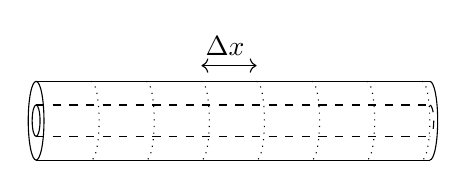
\begin{tikzpicture}
	\draw (2.4,0.7) node[above] {$\Delta x$};
	\draw[<->] (2.1,0.7) -- (2.8,0.7);
	\draw (0,0) ellipse(0.1 and 0.5);
	\draw (0,0) ellipse(0.05 and 0.2);
	\draw (0,0.5)--(5,0.5);
	\draw (0,-0.5)--(5,-0.5);
	
	\draw[dashed] (0,0.2)--(5,0.2);
	\draw[dashed] (0,-0.2)--(5,-0.2);
	\draw[dotted] (0.7,0.5) arc(90:-90:0.1 and 0.5);
	\draw[dotted] (1.4,0.5) arc(90:-90:0.1 and 0.5);
	\draw[dotted] (2.1,0.5) arc(90:-90:0.1 and 0.5);
	\draw[dotted] (2.8,0.5) arc(90:-90:0.1 and 0.5);
	\draw[dotted] (3.5,0.5) arc(90:-90:0.1 and 0.5);
	\draw[dotted] (4.2,0.5) arc(90:-90:0.1 and 0.5);
	\draw[dotted] (4.9,0.5) arc(90:-90:0.1 and 0.5);
	\draw (5,0.5) arc(90:-90:0.1 and 0.5);
	\draw[dashed] (5,0.2) arc(90:-90:0.05 and 0.2);
\end{tikzpicture}
\caption{}
\end{subfigure}
\begin{subfigure}[c]{0.4\textwidth}
\begin{circuitikz}
	\draw[dashed] (1,0) -- (2,0);
	\draw[dashed] (6,0) -- (7,0);
	\draw (2,0) to[L,*-*] (4,0) to[L,-*] (6,0) ;
	\draw (2,0) to[C] (2,-2) node[below] {$x_{n-1}$};
	\draw (4,0) to[C] (4,-2) node[below] {$x_n$};
	\draw (6,0) to[C] (6,-2) node[below] {$x_{n+1}$};
	\draw[dashed] (1,-2)--(2,-2);
	\draw (2,-2)--(6,-2);
	\draw[dashed] (6,-2)--(7,-2);
	
	%labes
	\draw (1,-1) node[right] {$C$} ;
	\draw (3,-1) node[right] {$C$} ;
	\draw (5,-1) node[right] {$C$} ;
	\draw (3,-0.4) node {$L$};
	\draw (5,-0.4) node {$L$};
	
	% currents
	\draw (3,0.5) node {$I_n$};
	\draw (5,0.5) node {$I_{n+1}$};	
\end{circuitikz}
\caption{$x_{n+1}-x_n = \Delta x$}
\end{subfigure}

\end{figure}


The potential difference of the $n$-th inductor is
\begin{equation}
	-V_n = \varphi_{n-1} - \varphi_n = L \dt{I_n}, 
\end{equation} 
where $f_n = f(x_n,t)$. The potential difference in the $n$-th capacitor is $\varphi_n = \frac{Q_n}{C}$ and has a current $\dt{Q_n}$. Taking the derivative of the potential and using KCL we get
\begin{equation}
	\dt{\varphi_n} =\frac{1}{C}\dt{Q_n} = \frac{1}{C}(I_n-I_{n+1})
\end{equation}
thus
\begin{equation}
	\dt{\varphi_{n-1}} - \dt{\varphi_n} = L \frac{d^2 I_n}{dt^2} 
\end{equation}
substuting , we get
\begin{equation}
	\frac{1}{C} (I_{n-1} -I_n) - \frac{1}{C}(I_n-I_{n+1}) = L \frac{d^2 I_n}{dt^2}
\end{equation}

Finally we arrive at
\begin{equation}
	\frac{\partial^2 I}{\partial x^2} - \frac{1}{v^2}\frac{\partial^2 I}{\partial t^2} = 0
\end{equation}
where $v^2 = \frac{(\Delta x)^2}{LC} = c^2$.

\textbf{Mutual inductance}\\
Consider a cilinder made by a material with permeability $\mu$, radius $a$ and length $l\gg a$. Roll a cable around the cilinder with $N\gg 1$ turns and set a current $I_1$, call this configuration circuit 1. Roll a second cable aorund the cilinder, but isolated from the first one, with $N_2 \gg 1$ turns and a current $I_2$, call it circuit 2. Then the magnetic field is
\begin{equation}
	B = B_1 + B_2 = \frac{4\pi}{c}\frac{N_1}{l}I_1 + \frac{4\pi}{c}\frac{N_2}{l}I_2
\end{equation}
and the energy density
\begin{equation}
	u = \frac{BH}{8\pi} = \frac{\mu}{8\pi}\left(\frac{4\pi}{cl} \right)^2 (N_1 I_1 + N_2 I_2)^2
\end{equation}
integrating over the volume of the cilynder we get the total energy
\begin{equation}  
	U = \frac{2\pi}{c^2 l^2}\mu (\pi a^2 l)(N_1 I_1 + N_2 I_2)^2 = \frac{2\pi^2 a^2}{c^2 l}\mu (N_1^2 I^2_1 + 2N_1N_2 I_1 I_2 + N_2^2 I_2^2)
\end{equation}
Changing notation
\begin{equation}
	U = \frac{1}{2} \sum_{ij}L_{ij}I_iI_j,\ \ \ i,j =1,2
\end{equation}
where
\begin{equation}
	L_{ii} =  \frac{4\pi^2 a^2}{lc^2}\mu N_i \text{  (no implicit sum), } L_{12} = L_{21} =  \frac{4\pi^2 a^2}{lc^2}\mu N_1N_2
\end{equation}
We realize that $L_{ij} = L_{ji}$ with $i\ne j$. The power of the coil is the derivative w.r.t. time, then
\begin{equation}
	\dt{U} = \mathcal{P} = \sum_{ij}I_i L_{ij}\dot{I}_j
\end{equation}
Also, the power is the work per unit time we do over the charges over $I_1$ plus, the work over $I_2$
\begin{equation}
	\mathcal{P} = \sum_{ij}\dt{q_i} L_{ij} I_j
\end{equation}
I we move a charge from one point to another, it will lose energy which is gained by the coil, then
\begin{equation}
	\mathcal{P} = \sum_i \dt{q_i} V_i
\end{equation} 
Comparing, we get
\begin{equation}
	V_i = \sum_{j} L_{ij}I_j
\end{equation}
We call $L_{ii}$ (no implicit sum) the \textit{autoinductance}. And $L_{ij}$, with $i\neq j$ \textit{mutual inductance}.


\textbf{Transformers}\\
Consider the circuit in figure ... Since it is an open circuit $I_2 = 0$ and using eq.  
\begin{eqnarray}
	V_1 & = & L_{11}\dt{I_1} \\
	V_2 & = & L_{21}\dt{I_2}
\end{eqnarray}
Then
\begin{equation}
	\frac{V_2}{V_1} = \frac{L_{21}}{L_{11}} \Rightarrow V_2 = \frac{L_{21}}{L_{11}} V_1 \Rightarrow V_2 = \frac{N_{2}}{N_{1}} V_1
\end{equation}
Now we close the circuit with a resistor $R_C$. We suppose a voltage source that provides with an amplitude $V_{10}$ and a frequency $\omega$. We write the voltage and the current represented by the real part of
\begin{eqnarray}
	V_1(t) & = & V_{10}e^{-i\omega t} \\
	I_1(t) & = & I_{10}e^{-i\omega t}
\end{eqnarray}
After some time we can also write the current in the second circuit as
\begin{equation}
	I_2(t)  =  I_{20}e^{-i\omega t}
\end{equation}
Using eq. and Ohm's law, we get the set of couple equations
\begin{eqnarray}
	V_1 & = & -i\omega L_{11}I_1 -i\omega L_{12}I_2 \\
	V_2 & = & -i\omega L_{21}I_1 -i\omega L_{22}I_2 \\
	V_2 & = & R_C I_2 
\end{eqnarray}
Now suppose $R_C$ is large in order to $I_2$ to be really small. Then we can dismiss the terms containing $I_2$ so we can use eq.
\begin{equation}
	I_2 \approx \frac{L_{21}}{L_{11}} \frac{V_1}{R_C}
\end{equation}
Another situation is when $R_C = 0 \Rightarrow V_2 = 0$. Then circuit 2 is in short-circuit. This gives constraints, $I_1$ must not be too large in order for  circuit 2 not to burn. 

\textbf{More on Conservation Laws}\\
We know that $\vec{j}\cdot \vec{E}$ is the power per unit time per unit volume that the fields give to a mechanical system. Therefore $-\vec{j}\cdot \vec{E}$ is power the system gives to the fields. We can interpret this as the source of energy density of the fields. Then the energy density of the fields satisfy the a continuity equation with sources
\begin{equation}
	-\vec{j}\cdot \vec{E} = \partial_t u + \nabla \cdot \vec{S}
\end{equation}
where $u$ is the energy density and $\vec{S}$ is the flow of energy. We can substitute $\vec{j}$ in the LHS using Ampere's law, then
\begin{eqnarray}
	-j_iE_i & = & -\frac{c}{4\pi}\epsilon_{ijk}(\partial_j B_k)E_i + \frac{1}{4\pi}(\partial_t E_i)E_i \\
	& = & - \frac{c}{4\pi}\partial_j (\epsilon_{ijk}B_k E_i) + \frac{c}{4\pi}\epsilon_{ijk}B_k\partial_j E_i + \frac{1}{8\pi}\partial_{t}(E_iE_i) \\
	& = & \partial_j \left( \frac{c}{4\pi} \epsilon_{ijk}E_i B_k\right) -\frac{c}{4\pi}(\epsilon_{kji}\partial_j E_i)B_k + \frac{1}{8\pi}\partial_t (E_iE_i)\\
	& = & \partial_j \left( \frac{c}{4\pi} \epsilon_{ijk}E_i B_k\right) + \partial_t \frac{1}{8\pi} (E_iE_i + B_iB_i) \\
	& = & \partial_t u + \nabla \cdot \vec{S}
\end{eqnarray}
where
\begin{eqnarray}
	u & = & \frac{1}{8\pi} (E^2 + B^2) \\
	\vec{S} & = & \frac{c}{4\pi}\vec{E} \times \vec{B}
\end{eqnarray}
In materials, the energy must satisfy a contonuity equation with sources, but now the current density  is the current that does not come from the materials. We call it the external current density $\vec{j}^{\text{ex}}$. So 
\begin{equation}
	-\vec{j}^{\text{ex}}\cdot \vec{E} = \partial_t u + \nabla \cdot \vec{S}
\end{equation}
With a similar analysis but now using Maxwell equations in materials we arrive at
\begin{eqnarray}
	u & = & \frac{1}{8\pi} (\vec{
	E}\cdot\vec{D} + \vec{B}\cdot \vec{H}) \\
	\vec{S} & = & \frac{c}{4\pi}\vec{E} \times \vec{H}
\end{eqnarray}
However these relations are only valid in no dispersive regions of transparency where we can assume both the permeability and permitivity as constants. 

\textbf{Conservation of momentum}\\
From Newton's 2nd law, the Lorenz force is$F_{\text{em}} = \dot{p}$ where $F_{\text{em}}$ is  the momentum per unit time that the fields give to a mechanical system, therefore $-F_{\text{em}}$ is the source of momentum per unit time given to the fields. Then the fields satisfy a continouity equation of momentum with source
\begin{equation}
	-\vec{f} = -\rho \vec{E} - \frac{1}{c}\vec{j}\times \vec{B} = \partial_t \vec{g} + \nabla\cdot(-T)
\end{equation}
where $\vec{g}$ is the momentum density and $-T$ is the flux of momentum. Using the component representation of the LHS and using Gauss' Law and Ampere's to substitute $\rho$ and $\vec{j}$ we arrive at
\begin{eqnarray}
	\vec{g} & = & \frac{1}{4\pi c} \vec{E}\times \vec{B} \\
	T & = & \frac{1}{4\pi} \left(\vec{E}\vec{E}+\vec{B}\vec{B}-\frac{1}{2}(E^2 + B^2)I\right)
\end{eqnarray}
\textbf{Stress Tensor}\\
$T$ is a symmetric tensor known as the \textit{Stress Tensor}.

\begin{tabular}{c}
$-T_{ij}$ :  $j$ component of momentum that flows over direction $i$ per unit time per unit area. 
\end{tabular} 

The stress tensor is useful to work with problems where the force is needed but there is a discontinuity of the fields.
From fluid mechanics we know that
\begin{equation}
	\vec{F}_V = \int d\vec{a}\cdot T
\end{equation}
is the force acting in the interior of a volume $V$. Imagine a surface that experience a pressure $p$ due to is inmeresed in a fluid. A chunk of surface $da$ feels a force that push it to the inside
\begin{equation}
	d\vec{f} = - p d\vec{a}
\end{equation}
thus
\begin{equation}
	\vec{F} = -\int d\vec{a} \ p = \int d\vec{a} \cdot (-pI)
\end{equation}
Therefore in a fluid $T = -p I$. This result let us interpret terms in the diagonal. Negative terms are pressures, and positve terms are tensions per unit area.

\textbf{Force on the plates of a capacitor}\\
Consider a capacitor where we glue a charge $Q$ on the left and $-Q$ on the right. What force is acting on the left plaque? We know that the field is discontinous. Outside the plaques the field is 0 and inside is $E = \frac{4\pi Q}{A}$. We could argue that the force on the left plaque is $F  = \frac{4\pi Q^2}{A}$. However, imagine that we move lightly to the left plaque 1 a distance $l$. In magnitude $F_{\text{me}} = F_{\text{e-m}}$, then we have produced work $W = F_{\text{me}} l = F_{\text{e-m}} l= \Delta U$, where $\Delta U$ is the change in potential energy and $\Delta U = \Delta V u = (A l)\frac{E^2}{8\pi}$,where $\Delta V$ is the change in the volume and $u$ is the energy density of the electric field. Therefore $F_{\text{e-m}} = \frac{2\pi Q^2}{A}$. Which is differente from the previous one, which is the correct one?. We use instead the momentum conservation equation. In a stationary situation $\partial_t\vec{g} = 0$ and
$-\vec{f} = -\nabla \cdot T$ so $\vec{F} = \int_{\partial V} d\vec{a}\cdot T$. The only non zero component of $T$ is 
\begin{equation}
	T_{xx} = \frac{1}{8\pi}E^2 
\end{equation}
thus
\begin{equation}
	F_x = \frac{1}{8\pi}E^2 A = \frac{2\pi Q^2}{A} = \frac{1}{2}Q E
\end{equation}
Therefore, the plaques are in tension.

\textbf{Force acting on the wires of a solenoid}\\
Consider a long solenoid of radius $a$ and length $l \gg a$.  We know that $\vec{B} = \frac{4\pi}{c}\frac{N}{l} I \hat{z}$, where $r<a$ and $\vec{B} = 0$ where $r>a$. We have a discontinuity in the field 

\textbf{Conservation of angular momentum}\\
We can consider $-\vec{r}\times \vec{f}=-\vec{\tau}$ to be the source of angular momentum per unit time per unit volume of the fields.
\begin{eqnarray}
	-\vec{r}\times \vec{f} & = & \vec{r}\times(\partial_t \vec{g} - \nabla\cdot T) \\
	-\vec{\tau}_i & = & \partial_t(\vec{r}\times\vec{g})_i  + \epsilon_{ijk}r_j\partial T_{lk} \\
	& = & \partial_t(\vec{r}\times\vec{g})_i + \partial_l (\epsilon_{ijk}r_jT_{lk}) - \epsilon_{ijk}(\partial_l r_j)T_{lk} \\
	& = & \partial_t(\vec{r}\times\vec{g})_i + \partial_l (\epsilon_{ijk}r_jT_{lk}) - \epsilon_{ijk}T_{jk}\\
	-\vec{\tau} & = & \partial_t \vec{l} + \nabla\cdot M
\end{eqnarray}
where 
\begin{eqnarray}
	\vec{l} & = & \vec{r}\times \vec{g}\\
	M_{li} & = & \epsilon_{ijk}r_j T_{lk}
\end{eqnarray}


\textbf{Particular solution to the wave equation in 3d with initial conditions}\\
Suppose we have a function $\Psi$ satisfying the wave equation with initial conditions
\begin{equation}
	\Psi(\vec{r},0) = 0, \ \ \ \partial_t \Psi(\vec{r},0) = V(\vec{r})
\end{equation}
We apply the fourier transform to the spatial component of $\Psi$, $\Psi(\vec{r},t) = \int{\frac{d^3k}{(2\pi)^3}}\  \Psi_{\vec{k}}(t)e^{i\vec{k}\cdot\vec
r}$ and to the wave equation wich turns $\nabla \rightarrow i\vec{k}$, therefore
\begin{equation}
-k^2 \Psi_{\vec{k}}(t) -\frac{1}{c^2}\partial_t^2\Psi_{\vec{k}}(t) = 0 \Rightarrow \der{^2\Psi_{\vec{k}}(t)}{t^2} = - c^2k^2\Psi_{\vec{k}}(t)
\end{equation}
so we get a solution
\begin{equation}
\Psi_{\vec{k}}(t) = a_{\vec{k}} \cos (\omega_k t) + b_{\vec{k}} \sin (\omega_k t), \ \ \ \omega_k = kc
\end{equation}
The initial conditions in fourier space are
\begin{equation}
	\Psi_{\vec{k}}(0) = 0 \Rightarrow a_{\vec{k}} = 0, \ \ \ \dt{\Psi_{\vec{k}}}(0) = V_{\vec{k}} = \integral{}{}{^3r} V(\vec{r})e^{-i\vec{k}\cdot\vec{r}} \Rightarrow  b_{\vec{k}} = \frac{V(\vec{k})}{kc}
\end{equation}
thus
\begin{equation}
\Psi(\vec{r},t) = \int d^3 r' \ V(\vec{r'}) \int \frac{d^3k}{(2\pi)^3}\ \frac{\sin (kct)}{kc} e^{i\vec{k}\cdot(\vec{r}-\vec{r}')}  
\end{equation}
To evaluate the integral we use spherical coordinattes. We choose the $z$ axis in the $\vec{r}-\vec{r}'$ direction, so $\vec{k}\cdot(\vec{r}-\vec{r}') = k|\vec{r}-\vec{r}'|\cos \theta$, we also write $\vec{R} = |\vec{r}-\vec{r}\,'|\hat{\Omega}$ 
\begin{eqnarray}
	%\Psi(\vec{r},t) & = & -\frac{1}{4c}\int d^3r' \ \frac{V(\vec{r}\,')}{R} \int_{-\infty}^{\infty} \frac{dk}{(2\pi)^2} \left(e^{ik(R+ct)} - e^{-ik(R-ct)}+e^{-ik(R-ct)} + e^{-ik(R+ct)}\right) \nonumber\\
	\Psi(\vec{r},t)& = & -\frac{2}{4c} \frac{1}{2\pi} \int d^3r' \frac{V(\vec{r}\,')}{R} \left[\delta(\underbrace{R+ct}_{>0}) - \delta(R-ct) \right]
\end{eqnarray}
We are only considering times greater than $t = 0$, where the initial conditions are, so we can drop $\delta(R+ct)$. And 
\begin{equation}
	\Psi(\vec{r},t) = \frac{1}{4\pi c} \int d^3r' \  \frac{V(\vec{r}\,')}{|\vec{r}-\vec{r}\,'|} \delta(ct-|\vec{r}-\vec{r}\,'|)
\end{equation}
We replace the integral over $r'$ with $R$ so
\begin{equation}
	\Psi(\vec{r},t) = \frac{t}{4\pi} \int d\hat{\Omega} \ V(\vec{r} + ct\hat{\Omega}) = t \langle V(\vec{r} + ct\hat{\Omega}) \rangle_{\hat{\Omega}}
\end{equation}

\textbf{General solution of the wave equation in 3d with initial conditions}\\
Suppose we have a function $\Psi$ satisfying the wave equation with initial conditions
\begin{equation}
	\Psi(\vec{r},0) = I(\vec{r}), \ \ \ \partial_t \Psi(\vec{r},0) = 0
\end{equation}
If we define the function $\varphi(\vec{r},t) =t \langle I(\vec{r} + ct\hat{\Omega}) \rangle_{\hat{\Omega}}$, which satisfies the wave equation with initial conditions 
\begin{equation}
	\varphi(\vec{r},0) = 0, \ \ \ \partial_t \Psi(\vec{r},0) = I(\vec{r})
\end{equation}
we verify that $\Psi(\vec{r},t) = \partial_t \varphi(\vec{r},t)$. Finally, if we have a function satifying the wave equation with generic initial conditions
\begin{equation}
	\varphi(\vec{r},0) = I(\vec{r}), \ \ \ \partial_t \Psi(\vec{r},0) = V(\vec{r})
\end{equation}
we arrive at the solution
\begin{equation}
	\Psi(\vec{r},t) = t \langle V(\vec{r} + ct\hat{\Omega})\rangle_{\hat{\Omega}} + \pd{}{t} t \langle I(\vec{r} + ct\hat{\Omega})\rangle_{\hat{\Omega}}
\end{equation}

\textbf{Turning on a field adiabatically}\\
The sources in Maxwell's equations are ones that have existed always. In reality, the sources are turn on at some time and the turned off at some later time.
Consider a source $f(t) = \int \frac{d\omega}{2\pi}f_{\omega}e^{-i\omega t}$, this tells us that a source is a superposition of waves that have osicillated from $t\to-\infty$ and will keep oscillating to $t\to+\infty$ which is not realistic.



\textbf{Spatial and time translational invariance in the Green's function}\\
Greens' functions have a traslation invariance if we move rigidly the source and the point of measure. Also, they have time translational invariance since  the effect at time $t$ of a source produced at time $t'<t$ only depend on the time difference. In this sense
\begin{equation}
	G(\vec{r},\vec{r}\,',t,t')= G(\vec{r}+ \vec{a},t+t_0,\vec{r}\,'+\vec{a},t'+t_0) 
\end{equation}   
In particular we can choose $\vec{a} = -\vec{r}\,'$ and $t_0 = -t'$ so now the Green's function only depend on just two variables $\vec{r}-\vec{r}\,'$ and $t-t'$ 
\begin{equation}
	G = G(\vec{r}-\vec{r}\,',t-t')
\end{equation}

\textbf{Solution to the wave equation with sources in 3d}\\
Suppose $\Psi(\vec{r},t)$ satisfies the wave equation with sources
\begin{equation}
	\nabla^2 \Psi - \frac{1}{c^2}\partial_t^2 \Psi = -4\pi f 
\end{equation}
We guess a Green's function $G$ to be the solution of a wave equation with a point source at $\vec{r}\,'$ that only live at time $t'$ (obviuosly not real since sources/charges are conserved)
\begin{equation}
	\left( \nabla^2 - \frac{1}{c^2}\partial_t^2\right)G(\vec{r},t,\vec{r}\,',t') = - 4\pi \delta(\vec{r}-\vec{r}\,')\delta(t-t')
\end{equation}
so that
\begin{equation}
	\Psi(\vec{r},t) = \int d^3r' \int dt' \ G(\vec{r}-\vec{r}\,',t-t') f(\vec{r}\,',t')
\end{equation}


Now we do $\vec{r}-\vec{r}\,' \to \vec{r} $  and $t-t' \to t$ and the equation for $G$ reads
\begin{equation}
	\left( \nabla^2 - \frac{1}{c^2}\partial_t^2\right)G(\vec{r},t) = - 4\pi \delta(\vec{r}\,)\delta(t)
\end{equation}
Applying fourier transform and solving we get
\begin{equation}
	G_{\vec{k}\omega} = \frac{4\pi}{k^2 - \frac{\omega^2}{c^2}}
\end{equation}
Therefore
\begin{equation}
	G(\vec{r},t) = -4\pi c^2 \int \frac{d^3k}{(2\pi)^3}\int \frac{d\omega}{2\pi} \ \frac{1}{(\omega + kc)(\omega -kc)}e^{i(\vec{k}\cdot\vec{r}-\omega t)}
\end{equation}
In order to evalute integral over $\omega$ we turn $\omega$ into a complex number $\omega = \omega' + i\omega''$ in this way we can use Cauchy's residue theorem.  However we have two poles $\omega = \pm kc$ we need to avoid. We invoke the causality principle: sources now ($t = 0$) do not affect the field in the past ($t<0$). This means that the integral at times $t<0$ must vanish. One way to warranty that the reponse is causal, is to assure there are no singularities inside the countour.
%These kind of integral often use a contour of a semi-circle going up or down.
If we want integral over the semicircle to vanish at $R\to\infty$ we need to have $e^{\omega''t}<1$ this means $\omega'' > 0$. 
 If we turn the sources adiabatically, that is we write $\omega \to \omega+ i\eta, \ \eta >0, \ \eta \to 0^+$, then we would have moved the poles down to the imaginary axis by $\eta$, that is $\omega = \pm kc - i\eta$. From Cauchy's theorem the integral over the upper semicircle will vanish sincce there are no poles enclosed.   

If $t>0$ we use Cauchy's theorem with a countour as in figure ...
Then we get

\begin{equation}
	G(\vec{r},t) = -4\pi c^2 \int \frac{d^3k} {(2\pi)^3}\ e^{i\vec{k}\cdot\vec{r}} \frac{-2\pi i}{2\pi}\left[\frac{e^{-ikct}}{2kc}+ \frac{e^{ikct}}{-2kc}\right]
\end{equation}
	
\end{document}